%!TEX root = series of tubes.tex

\section{The Design Space of Pipes}
Our review of prior art indicates the potential benifits of using interior pipes for adding interactivity to 3D printed objects, although no general purpose tools currently exist for this purpose. To guide the design of such tool, we now provide a design space of the types of pipes that a maker may want to utilize. We have identified four relevant dimensions of pipe design: \emph{openings}, \emph{path constraints}, \emph{topologies}, and inserted \emph{media}.  We describe the space (see Figure \ref{fig:pipespace}) below.

\begin{figure}[t]
\centering
    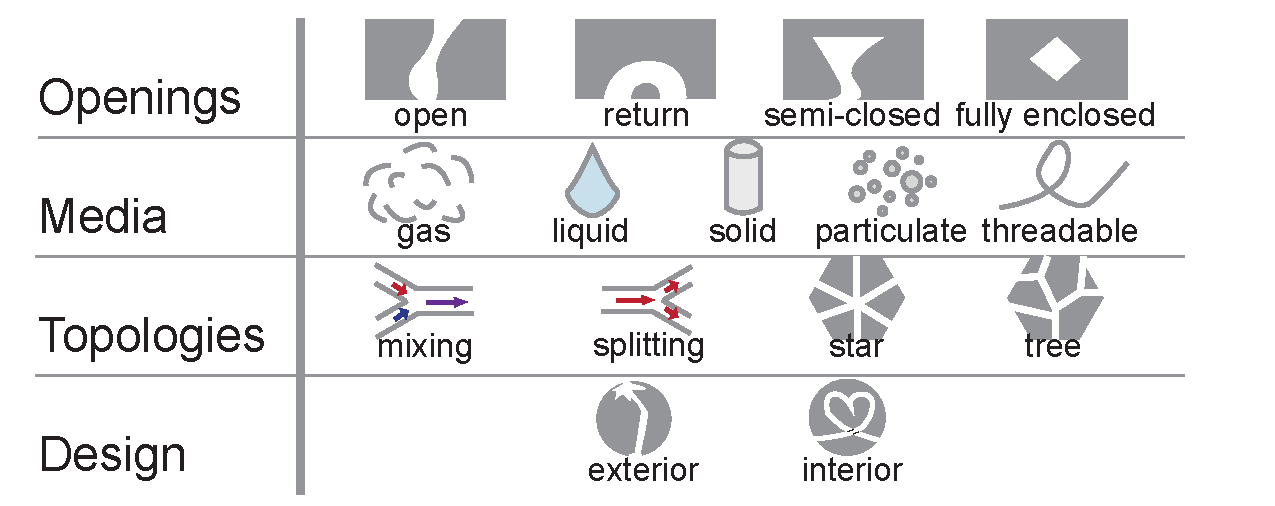
\includegraphics[width=1.0\columnwidth]{figures/tubespace.pdf}
\caption{The design space of pipes.  Pipe \emph{openings}, \emph{path constraints}, \emph{topologies}, and inserted \emph{media} give rise to unique input/output possibilities.}
\label{fig:pipespace}
\end{figure}

\subsection{Openings}
Pipes inside solid objects can be either \emph{open} to the outside on both ends, \emph{semi-enclosed}, or \emph{fully enclosed} (see Figure \ref{fig:pipespace}). For interactive devices, openings can be either user-facing (in places a user would for example touch a model); or system-facing, where sensors and actuators may be connected.
%\george{difference between open/return not clear}
%Pipes can have four opening styles: open, return, semi-closed, and fully enclosed .  As we are interested in interactive devices, we distinguish a ``user side"---part of the surface or interior of an object facing its user for interaction; and a ``system side"---where other hardware such as electronics may be connected.  We refer to a pipe which is ``open on the user side'' to have its contents \emph{physically accessible} to a user \emph{at interaction time}.  ``Closed on the user side'' implies physically cut off from the user.  Similarly with the system side.  User or system manipulation of pipe contents are possible even without physical access: e.g., via soundwaves. \george{confusing}

\begin{figure}[t]
\centering
    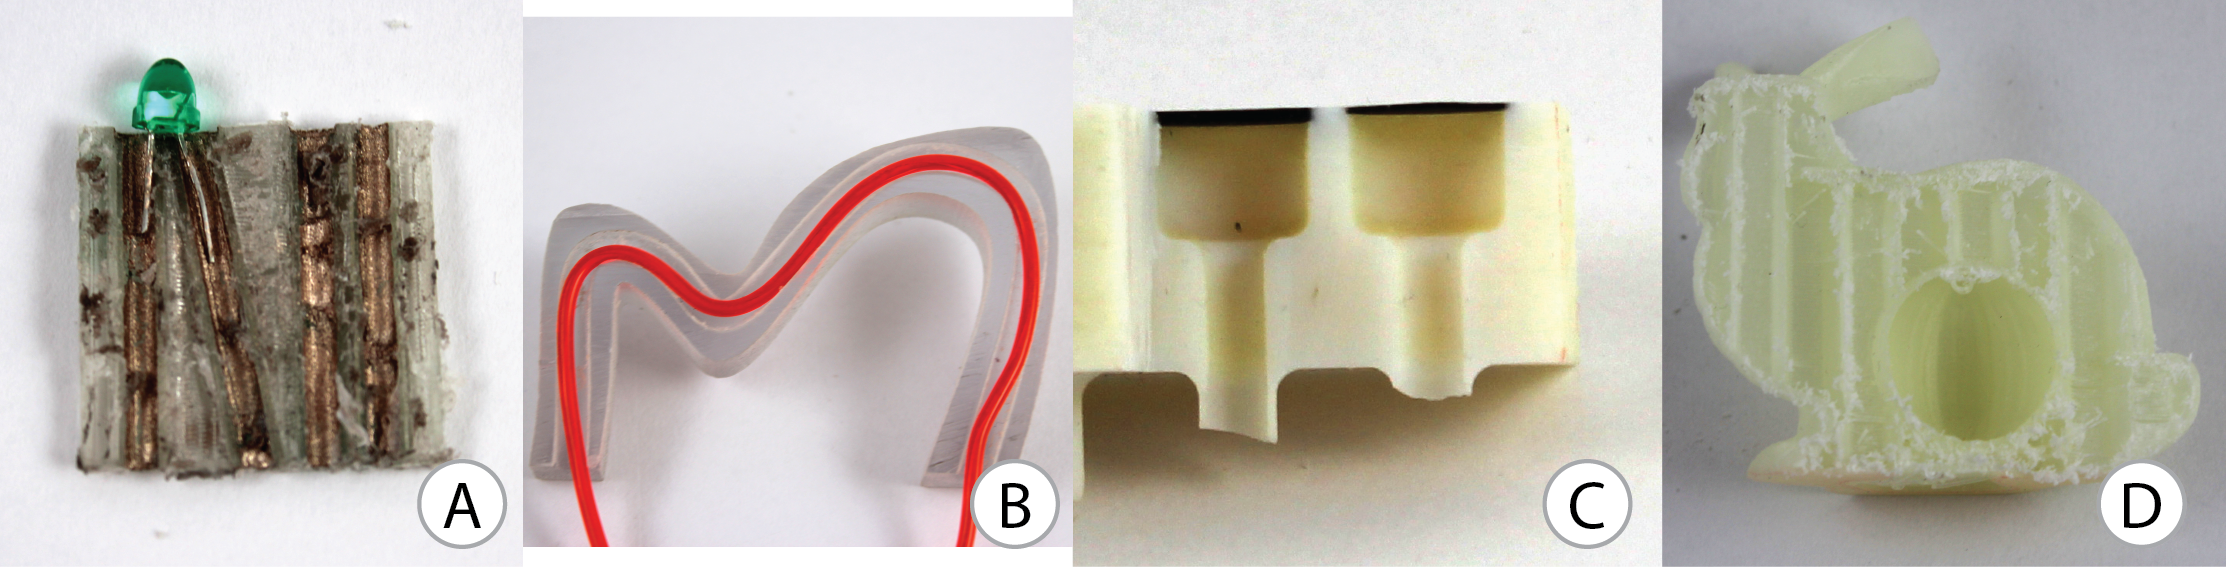
\includegraphics[width=1.0\columnwidth]{figures/types.png}
\caption{Pipe openings: A shows a pair of \emph{open} pipes filled with copper paint to power an LED.  B shows two \emph{semi-closed} pipes capped by rubber membranes.  In C, a rabbit has a \emph{fully enclosed} chamber to modify its weight.}
\label{fig:openings}
\end{figure}

\emph{Open} pipes may be used to create electronic circuitry.  For example, an open pipe filled with conductive paint and connected to a battery can provide power to an LED (see Figure \ref{fig:openings}a).
%
\emph{Semi-enclosed} pipes are capped on one side and could be used to create create tactile output. By fabricating a cap from a malleable material and attaching a pump to the open end, haptic feedback can be generated by raising and depressing the flexible cap (see Figure \ref{fig:openings}b).
%
\emph{Fully enclosed} pipes (cavities) are entirely internal to the object.  Fully enclosed pipes may be used as weight modifiers~\cite{Prevost-makeitstand} and for object identification~\cite{Willis-infrastructs}, as in Figure \ref{fig:openings}c.  If printed in parts and assembled post-print, enclosed pipes could also contain water or particles that would otherwise fall out.

\subsection{Path Constraints}
Depending on the purpose of the pipe, its geometry may be constrained to specific locations within the 3D model. An \emph{endpoint-constrained} pipe requires specific start and end points, but the particular route of the internal path is irrelevant. This is the case for circuit schematics, where the electronic components have a fixed location, but many routing solutions are valid. In contrast, for a \emph{path-constrained} pipe the shape of the path is important. For example, threading electroluminescent (EL) wire through a clear pipe enables makers to emulate neon art (see Figure \ref{fig:teaser}, right). A \emph{fully constrained} pipe requires both specific terminals as well as a specific path. If a maker wishes the EL wire to exit the rear of the sign to hide the electronics, she can use a fully-constrained path (Figure \ref{fig:neon}). Finally, an \emph{unconstrained} pipe does not need a specific path or terminal points. A cavity to modify an object's weight is an example of an unconstrained pipe.

\subsection{Pipe Topologies}
Pipe network topologies enable \emph{splitting} or \emph{mixing} of media (see Figure \ref{fig:pipespace}).  \emph{Star} and \emph{tree} topologies extend the splitting and mixing primitives, encompassing multiple-in and multiple-out configurations; we use star topologies to create different sensing location for our touch-sensitive toys, with one terminal used for swept-frequency capacitive sensing (Figure~\ref{fig:examples}a).

\subsection{Media in Pipes}
After printing, different media can be inserted into pipes to change affordances and capabilities. We consider \emph{gas}, \emph{liquids}, \emph{solids}, \emph{particulates}, and \emph{threadables}. 
%
Compressible fluids (\emph{``gas''}) and incompressible fluids (\emph{``liquids''})  inside semi-enclosed pipes can create haptic feedback; pressure can also be sensed to act as an input~\cite{Slyper-shape}. Gases can be used as carriers for scents or fog. Conductive liquids like copper paint, when dried, turn pipes into conductive paths and can also fix electronic components in place.
%
Filling pipes with \emph{solids} at print time enables designers to exploit the difference in material properties between pipe and contents. For example, in Printed Optics~\cite{Willis-printedoptics}, different refractive indices between solid cladding material and transparent material inside pipes allowed light transport along pipes for input and output.
%
\emph{Particulates}, either printed in-place or inserted, can be of varying densities and can contain particles of various and variable size.  A single large particle can be used for display.  Small particles in variable amounts of fluid can provide variable stiffness haptics via jamming \cite{Follmer-jamming}.
%
\emph{Threadable} media, such as regular wire, electroluminescent wire, or commercial fiberoptic cables, can be threaded through pipes post-printing. Threading such media enables addition of conduction, illumination, or optical sensing using materials that can easily be procured, but cannot themselves be printed, e.g., on consumer printers with a single material. 
% This empowers inexpensive printers: for example, a Printed Optics-style interface can be created on a consumer-grade 3D printer with pipes and fiber optic cable.

In the next section detail we how different pipes within this design space space can be created with the help of our new design tool, \systemnamenospace.
